\documentclass[11pt,a4paper]{article}
\usepackage[utf8]{inputenc}
\usepackage[T1]{fontenc}
\usepackage{lmodern}
\usepackage{amsmath,amssymb}
\usepackage{booktabs,multirow}
\usepackage{graphicx}
\usepackage{tikz}
\usetikzlibrary{arrows.meta,positioning,shapes.geometric}
\usepackage[hidelinks]{hyperref}
\usepackage[margin=2.5cm]{geometry}
\usepackage{natbib}

\title{Pravrudhi: Recursive Self-Improvement of Language-Model Systems under an Expected-Free-Energy Controller with Typed Evidence}
\author{Sharath Sathish}
\date{\today}

\begin{document}
\maketitle

\begin{abstract}
Recursive self-improvement systems for language-model harnesses share one skeleton and one epistemology: a mutable substrate, a proposer, a frozen evaluator, an archive, and the belief that a change is good if a number went up. This paper describes Pravrudhi, an engine that keeps the skeleton and replaces three components: selection by an expected-free-energy controller over a posterior held outside the language model; evidence typed by provenance and replaced only by sublation; and an evaluator kernel that the mutated process cannot reach. Results sections are filled from gate records as each experiment closes; this version reports the design and the measurement protocol.
\end{abstract}

% Source: docs/blueprint/README.md and 00-charter/CHARTER.md §1; no measured numbers.
\section{Introduction}
\label{sec:intro}

The industry state of the art in recursive self-improvement of language-model systems, from the Darwin G\"odel Machine lineage \citep{zhang2025dgm} to evolutionary program search and the autoresearch loops, is organised around a mutable substrate, a proposer, an evaluator that is assumed frozen, and an archive with a selection heuristic. The documented failures of that arrangement are failures of evidence rather than of search: fabricated test logs, removed hallucination markers, and kept changes that a paired comparison cannot distinguish from noise. Pravrudhi retains the skeleton and changes the three components that produce those failures. Selection becomes an expected-free-energy objective over a hierarchical posterior that is maintained outside the language model, so that each experiment is chosen for expected gain and expected information gain weighted by the proposer's earned calibration. Evidence becomes typed: every observation carries a provenance tag distinguishing kernel-executed measurement, surrogate inference, transfer analogy, and model testimony, and a stored claim is replaced only by a higher-precision defeat with a recorded reason. The evaluator moves into a small kernel that the mutated process cannot address, which makes fabrication a matter of construction rather than of policing.

The engine is delivered as an installable package that a practitioner runs on a single consumer GPU over a model and a harness of their own. The contribution under test is the typed-evidence ordering and the epistemic term of the objective; the naming discipline that accompanies them is an audit convention and is not itself a claim.

% Source: docs/blueprint/01-research/01-sota-landscape.md; comparison axes only, no measured numbers.
\section{Background}
\label{sec:background}

Four lineages of recursive self-improvement are relevant. Archive-based self-modification of a coding agent evaluates whole-scaffold rewrites on a benchmark and keeps parents by score. Evolutionary program search applies population operators to code under a fixed evaluator. The autoresearch loops edit a single training file under a fixed wall-clock budget and keep a change if a validation metric improves. Self-play weight trainers optimise adapters against verifiable rewards. Table~\ref{tab:related} contrasts them on the axes that the present design changes: where the posterior over effects lives, whether evidence carries provenance, and whether the evaluator is reachable by the mutated process.

\begin{table}[t]
\centering
\caption{Recursive self-improvement lineages compared on the three components Pravrudhi changes. ``Reachable'' means the process being mutated can, in principle, write to the evaluator's inputs or outputs.}
\label{tab:related}
\begin{tabular}{lccc}
\toprule
\textbf{Lineage} & \textbf{Posterior} & \textbf{Typed evidence} & \textbf{Evaluator reachable} \\
\midrule
Archive self-modification & none (score archive) & no & yes \\
Evolutionary program search & none (population) & no & yes \\
Autoresearch keep-if-better & none & no & yes \\
Self-play adapter training & implicit in reward & no & partly \\
Pravrudhi & explicit, hierarchical, external & yes & no \\
\bottomrule
\end{tabular}
\end{table}

% Source: docs/blueprint/02-design/02-efe-controller-spec.md §1–§3, 08-memory-and-context.md §1, 06-evaluation-and-statistics.md §3–§4; no measured numbers.
\section{Method}
\label{sec:method}

\subsection{Loop and mutability tiers}
A night is a budgeted batch of cycles. Each cycle proposes a candidate, deliberates over the pool, executes the selected candidates in disposable sandboxes, observes the kernel's scores, and disposes by a sequential test. Four mutability tiers separate what may change from what may not: the kernel is immutable within an epoch, the ledger is append-only, the harness and adapters are mutable through a broker, and canonical artefacts change only by human promotion. Figure~\ref{fig:loop} shows the phases and the residency windows.

\begin{figure}[t]
\centering
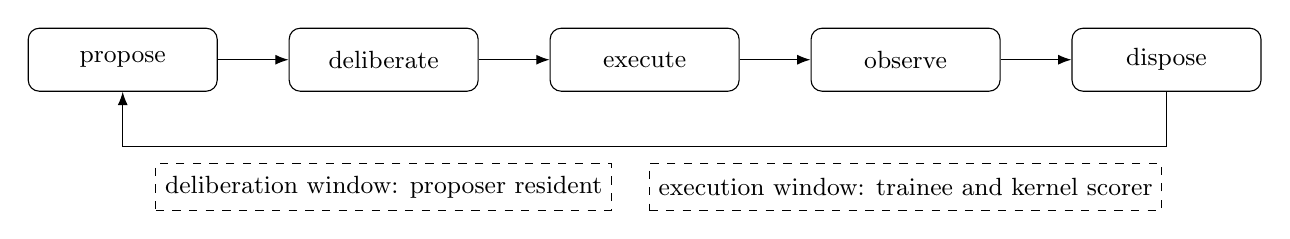
\begin{tikzpicture}[node distance=1.1cm and 0.9cm, every node/.style={font=\small}, box/.style={draw, rounded corners, minimum width=2.4cm, minimum height=0.8cm, align=center}]
\node[box] (p) {propose};
\node[box, right=of p] (d) {deliberate};
\node[box, right=of d] (e) {execute};
\node[box, right=of e] (o) {observe};
\node[box, right=of o] (s) {dispose};
\draw[-Latex] (p) -- (d); \draw[-Latex] (d) -- (e); \draw[-Latex] (e) -- (o); \draw[-Latex] (o) -- (s);
\draw[-Latex] (s.south) |- ++(0,-0.7) -| (p.south);
\node[below=0.9cm of d, draw, dashed, minimum width=5.6cm, minimum height=0.6cm] {deliberation window: proposer resident};
\node[below=0.9cm of o, draw, dashed, minimum width=5.6cm, minimum height=0.6cm] {execution window: trainee and kernel scorer};
\end{tikzpicture}
\caption{One night: the five phases, and the two residency windows on a single GPU. The kernel writes every observation; the engine never does.}
\label{fig:loop}
\end{figure}

\subsection{Objective}
For a candidate $a$ with evidence plan $\pi$, the controller scores the expected free energy $G(a,\pi) = -\gamma_{\mathrm{epi}}\,\mathrm{EIG}(a,\pi) - \gamma_{\mathrm{prag}}\,\mathbb{E}[\log p(o \mid C)] + \kappa\, c(a,\pi)$, where EIG is the expected information gain about the effect-size hierarchy, the pragmatic term is the expected log preference under prior preferences $C$ that assign $-\infty$ to any candidate touching the kernel, and $c$ is the cost in GPU-hours scaled by the residency phase. Precisions $\gamma$ are inferred from the ledger with a hard floor on the epistemic weight. The proposer's prediction enters the posterior as a pseudo-observation whose variance is inflated by the inverse of the proposer's calibrated reliability.

\subsection{Typed evidence and sublation}
Every ledger row carries a provenance tag from the set of kernel-executed measurement, surrogate inference, transfer analogy, and model testimony. A stored claim is replaced only when the replacing evidence has strictly higher precision on a common scale or an arbitration rule applies: specific over general, stronger provenance over weaker, later measurement over earlier inference. Refusals are logged.

\subsection{Selection arms}
The controller's value is a comparative claim, so the engine implements the arms it is compared against rather than
only the arm it advocates. A selection policy decides two things and nothing else: the order in which live
candidates are considered, and how the night's budget is filled. Everything downstream is held identical across
arms, including the pairing of candidate and incumbent on the same held-out rotation and sampling seed, the
sequential boundary, the canaries and the shape of every ledger row, so a difference between arms can only come
from selection. The expected-free-energy arm keeps the full apparatus: the habit prior, the sampling over the
softmax of the negative free energy, the reservation of budget for the highest-information candidate and the
planted and sensor shares. The baselines deliberately receive none of it. A greedy ratchet ranks by the posterior
mean, which is the best estimate of a candidate's effect the loop holds at that moment, and takes what currently
looks best; a ratchet that reserved budget for the most informative candidate would not be a ratchet. A lineage
Thompson sampler draws once from each candidate's posterior and ranks by the draw, so a wide posterior can win. A
random arm ignores the evidence entirely and is the null. Because the baselines run behind the same sequential
gate, the comparison isolates selection from gating, which is the arm the pre-registration names for that purpose.

The decorative-controller check, which asks whether the scores condition on the action at all, applies only to the
expected-free-energy arm and is recorded as inapplicable for the others: a baseline computes no such scores, and
the random arm is decorative by construction, which is precisely why it is included. Every selection row and every
night's opening row records the arm that produced it, so a ledger containing several arms remains analysable, and
the rendered comparison refuses to report a result at all when any arm received no paired evaluation.

\subsection{Recursion}
A night does not start from the base model. The night's reference is the latest promoted candidate for the trainee, read from the ledger's promotion rows and located through the training row that produced its adapter; every paired comparison of the night is against that incumbent, and the night's opening row records which one. Two channels carry the incumbent into the next generation on the weight target. In the first, the incumbent is the sampling teacher: it generates completions for training questions, the kernel's checker keeps the verified ones, and the candidate is fine-tuned on that set. In the second, a candidate continues the incumbent's adapter with its own data and optimiser settings rather than starting from the base weights; the adapter shape then follows the incumbent, and the recipe's shape parameters are recorded but not applied. A candidate that asks to continue the incumbent when the incumbent is the base model falls back to the base with an audit row, so lineage is never implicit. On the harness target the same rule holds with the promoted scaffold as reference. Merging a promoted adapter into the base checkpoint remains a human act through the inbox.

\subsection{Withdrawn observations}
An observation that was measured correctly but against the wrong reference is not deleted, since the chain is append-only, and is not left in the posterior either. A sublation row naming the observation's sequence number withdraws it: replay collects the withdrawn numbers in a first pass and skips those rows when it rebuilds each candidate's stream, while the rows, the sublation and its stated reason stay in the chain. The same mechanism serves any later correction of an admitted observation.

\subsection{Kernel isolation}
The kernel is a separate package with no model client and no network access. Observations are admissible only after the kernel verifies the hashes of the held-out items, the pool manifest, the scorer, the artefact under test, and the model weights inside the execution container. The isolation level that produced an observation, whether a separate process, a container, or a separate operating-system user, is recorded on the row.

\subsection{Product surface}
The engine is operated through six commands. \texttt{init} creates the kernel state directory with a private secret, installs the pre-registration files and prompt templates, and writes the genesis row of the ledger. \texttt{preflight} and \texttt{study noise-floor} measure the card and the unmodified model before any candidate exists. \texttt{night} runs one budgeted cycle of proposal, deliberation, execution and disposal. \texttt{inbox} lists what the night promoted, each entry carrying a badge derived by replaying the ledger, and \texttt{export} copies the promoted adapter with a provenance manifest that names the candidate, the ledger head and the adapter hash; it refuses any candidate whose badge is not green. \texttt{serve} exposes the same views over HTTP, and its only write, the operator's sign-off, refuses agent identities. A Claude Code plugin wraps these commands as skills so that an agent session can drive a project while the decision to promote stays with a person.


% Source: docs/superpowers/specs/2026-09-04-pravrudhi-engine-design.md §3, §6; 06-evaluation-and-statistics.md §3–§4. Protocol only; numbers arrive with gates L3–L4.
\section{Evaluation protocol}
\label{sec:evaluation}

The first target is adapter-only self-improvement of a four-billion-parameter open model on a grade-school arithmetic benchmark with a deterministic answer checker. The train split supplies the proposer's data; the test split is sealed as the held-out pool from which the kernel draws rotations under an exposure cap; a disjoint slice of the train split is the in-loop evaluation set. Candidates are bucketed by edit family so that the hierarchical posterior has between-family variance. Before any candidate is selected, the unmodified model is evaluated across rotations and sampling seeds to measure the evaluation noise floor; this noise floor fixes the sequential boundaries and the surprise threshold. Claims are stated at the tier they passed: smoke, screen, or confirm. A confirm-tier claim requires at least three seeds, a paired design, a bias-corrected bootstrap interval on Hedges' $g$, and family-wise correction at family closure.

% Source: gates/gate_L3.json (domain_gate.evidence), research/prereg/variance_v1_gsm8k-test_qwen3-4b.json, research/prereg/measured_stack_v1_qwen3-4b.json (archived L3 files; variance.json now holds the current trainee). Every number below is a field of one of these files.
\section{Results}
\label{sec:results}

\subsection{Execution spine and the measured noise floor}
\label{sec:results-l3}

The first evidence the kernel admitted is an A/A study of the unmodified trainee, run before any candidate existed, so that the sequential boundaries and the surprise threshold rest on a measured floor rather than a quoted one. Each run is a kernel-launched container job over one held-out rotation of 100 items drawn by keyed hash from the sealed pool of 1319 GSM8K test items under an exposure cap of three, with one sampling seed at temperature 0.7 and at most 512 new tokens. The container receives questions only; the kernel scores the completions against the sealed answers; an observation exists only after the item file, pool manifest, scorer source, artefact tree and model weights hash to the values the kernel sealed. Table~\ref{tab:l3-stack} records the stack as measured by the preflight job on the card used, and Table~\ref{tab:l3-noise} the study.

\begin{table}[t]
\centering
\caption{Execution stack as measured by the preflight job (32 items, batch 16, greedy, 256 new tokens). Throughput is batched decode; single-stream throughput is lower.}
\label{tab:l3-stack}
\begin{tabular}{ll}
\toprule
\textbf{Quantity} & \textbf{Measured} \\
\midrule
GPU & NVIDIA GeForce RTX 5090 (32607 MiB) \\
Image lineage & NVIDIA PyTorch 25.06; torch 2.8.0a0, CUDA 12.9, transformers 5.13.0 \\
Trainee & Qwen/Qwen3-4B, bfloat16 \\
Peak VRAM (driver / allocator) & 9.78 GiB / 8.595 GiB \\
Batched decode throughput & 494.6 tokens/s \\
Model load time & 0.86 s \\
\bottomrule
\end{tabular}
\end{table}

\begin{table}[t]
\centering
\caption{Noise floor of the unmodified trainee on the sealed pool: 10 rotations $\times$ 3 seeds $\times$ 100 items (3000 scored items), temperature 0.7, isolation level container. Wilson interval on the pooled pass rate.}
\label{tab:l3-noise}
\begin{tabular}{lc}
\toprule
\textbf{Quantity} & \textbf{Value} \\
\midrule
Pooled pass rate & 0.8997 \\
Wilson 95\% interval & [0.8884, 0.9099] \\
$\sigma_{\mathrm{seed}}$ (within rotation, between seeds) & 0.0212 \\
$\sigma_{\mathrm{rot}}$ (between rotation means) & 0.0304 \\
$\sigma_{\mathrm{total}}$ (all runs) & 0.0342 \\
Surprise threshold (99th percentile of $|z|$) & 2.373 \\
\bottomrule
\end{tabular}
\end{table}

Two consequences follow for the first night. The between-rotation dispersion exceeds the between-seed dispersion, so item sampling rather than decoding randomness dominates the variance of a 100-item pass rate; a paired design that evaluates candidate and incumbent on the same rotation and seed removes the larger component, and the sequential boundary is therefore parameterised on $\sigma_{\mathrm{seed}}$ with the minimum effect of interest set to twice that value. The pooled pass rate near 0.90 also bounds what an adapter can add on this benchmark: the headroom is about ten points, and an effect smaller than the seed noise cannot be distinguished at a single rotation, which the boundary's futility rule expresses as a prune carrying the label \emph{asiddha}.

\subsection{The first nights on the LoRA target}
\label{sec:results-l4}

% Source: gates/gate_L4.json (domain_gate.evidence, code_gate.evidence) and docs/evidence/L4_night1.md, L4_night2.md.
Two nights ran on the LoRA target with the pre-registered budget, the measured noise floor, and the proposer served locally. Across the nights the proposer emitted 29 recipes within the grammar, 15 by rejection-sampled supervised fine-tuning and 14 by group-relative policy optimisation; 18 were trained and evaluated in 29 paired comparisons against the incumbent on the same rotation and sampling seed, every one scored by the kernel after hash verification. The paired differences in pass rate had mean 0.001 and standard deviation 0.0201 over a range from $-0.040$ to $+0.050$. Under the sequential boundary parameterised on the measured seed noise, with the minimum effect of interest set to 0.0424, fourteen candidates were pruned with the label \emph{asiddha}, none crossed the efficacy boundary, and four remained under test when the sealed pool was exhausted after 39 rotations; nothing was promoted. Table~\ref{tab:l4-nights} summarises the account rendered from the ledger.

\begin{table}[t]
\centering
\caption{Nights 1 and 2 on the LoRA target (gsm8k-test, 100 items per rotation, one loop seed). Every entry is a field of the gate record or of the evidence documents rendered from the ledger.}
\label{tab:l4-nights}
\begin{tabular}{lc}
\toprule
\textbf{Quantity} & \textbf{Value} \\
\midrule
Recipes proposed (SFT / GRPO) & 29 (15 / 14) \\
Candidates trained and evaluated & 18 \\
Paired evaluations (candidate rows / incumbent rows) & 29 / 29 \\
Paired $\Delta$ pass rate: mean, SD, range & 0.001, 0.0201, [$-0.040$, $+0.050$] \\
Pruned (\emph{asiddha}) / confirmed / promoted & 14 / 0 / 0 \\
Continuing at pool exhaustion & 4 \\
GPU-hours charged (spend rows) & 1.804 \\
Scored predictions, mean Brier & 22, 0.195 \\
Predictor precision $\gamma_{\mathrm{prag}}$: first, last & 0.05, 0.896 \\
Strategy-switch rate (cumulative) & 24/54, Wilson [0.320, 0.576] \\
\bottomrule
\end{tabular}
\end{table}

The result is a null at the screen tier and it is informative in two ways. First, the boundary behaved as designed: candidates whose paired differences sat inside the seed noise were pruned rather than promoted, and the one candidate with a large first draw ($+0.050$) was followed by two draws at zero and remained undecided. Second, the target has almost no headroom for the pre-registered effect: an unmodified model that passes about nine tenths of the items can gain at most ten points, and an effect of four points is a fifth of that, so the study measures the boundary's discipline more than any adapter's merit. The controller's machinery did what the design asked of it, including the rise of the predictor's earned precision from the floor to 0.896 as its sealed predictions were scored, and the strategy-switch rate shows that the epistemic term kept both strategies in play. The experiment that follows from this null, recorded in the gate as the spawned proposal, is a target with a base pass rate near one half and a held-out pool sized to the planned number of confirmations.


\subsection{A trainee with headroom: night 4 and the external tier}
\label{sec:results-p1}

% Source: docs/evidence/P1_summary_4.json, docs/evidence/L4_night4.md, docs/evidence/P1_external.md (ledger rows 717-718, 725), research/prereg/variance.json (Qwen3-0.6B on gsm8k-trainB), ledger row 587 (recipe of c-0045).
The null of the first nights was answered as the gate proposed: the target moved to a trainee with headroom and to a pool sized for confirmations. Night 3 kept the 1.7B trainee on a second sealed pool of 3500 GSM8K training items (rows 3500--6999, disjoint from every prompt the loop samples or trains on) and returned four continuing candidates, three of which were taken to 400-item confirmations of $+0.010$ $[-0.025, 0.040]$, $+0.015$ $[-0.020, 0.045]$ and $+0.0175$ $[-0.0175, 0.0475]$ (BCa intervals; paired permutation $p$ of 0.66, 0.46 and 0.36), a second null at the same instrument resolution. Night 4 changed the trainee to Qwen3-0.6B, whose A/A study on the same pool gave a pooled pass rate of 0.603 with $\sigma_{\mathrm{seed}}=0.0223$ over 15 runs, doubled the rotation to 200 items, and admitted a teacher model (Qwen3-4B) to the sampling stage of the rejection-sampled fine-tuning recipe, so that the proposer could distil rather than only self-sample. Table~\ref{tab:p1-night4} summarises the night from the ledger.

\begin{table}[t]
\centering
\caption{Night 4 on the LoRA target (Qwen3-0.6B, gsm8k-trainB, 200 items per rotation, exposure cap 4, temperature 0.7). Every entry is a field of the summary rendered from the ledger for night 4.}
\label{tab:p1-night4}
\begin{tabular}{lc}
\toprule
\textbf{Quantity} & \textbf{Value} \\
\midrule
Recipes proposed (SFT / GRPO) & 8 (4 / 4) \\
Candidates trained and evaluated & 8 \\
Paired evaluations (candidate rows / incumbent rows) & 13 / 13 \\
Paired $\Delta$ pass rate: mean, SD, range & $-0.004$, 0.0395, [$-0.065$, $+0.090$] \\
Pruned (\emph{asiddha}) / confirmed / promoted & 7 / 1 / 1 \\
GPU-hours charged to the night (spend rows, including its studies) & 0.968 \\
Controller: $\mathrm{cv}_G$ range, max MI (bits) & [0.78, 1.10], 0.518 \\
Strategy-switch rate (cumulative) & 48/97, Wilson [0.397, 0.593] \\
\bottomrule
\end{tabular}
\end{table}

The promoted candidate, c-0045, is a rejection-sampled supervised fine-tune with the teacher: 1024 kept samples under a diverse-correct filter, three epochs at learning rate $5\times10^{-5}$, a rank-8 adapter on the attention projections with $\alpha=16$ and dropout 0.1. Its first paired draw against the incumbent on a 200-item rotation was $+0.090$, which crossed the efficacy boundary at one seed because the minimum effect of interest for this trainee is $2\sigma_{\mathrm{seed}}=0.045$ and the draw is four seed deviations from zero; the canaries passed (anchor negative log-likelihood within its 3\,\% bound, distinct-2 above 0.9, length ratio within bounds) and the candidate was promoted. Seven later candidates were pruned against the stronger incumbent. A 400-item confirmation on a fresh rotation, run after the night with the same trainee and seed protocol, gave a paired difference of $+0.040$ with BCa interval $[-0.010, 0.0825]$, 52 wins against 36 losses over 312 ties, and paired permutation $p=0.111$: consistent with an effect near the minimum of interest and, at $n=400$, not on its own a detection.

The external tier settles what the internal instrument leaves open. Table~\ref{tab:p1-external} reports \texttt{lm-evaluation-harness} 0.4.9 on the full GSM8K test set (1319 items, five-shot, exact match under the strict extractor) for the base Qwen3-0.6B and for the same weights with the c-0045 adapter, both offline, same invocation, batch 32, bfloat16. The adapter raises strict exact match from 0.4086 to 0.4898, a gain of 0.081 with tool-reported standard errors of 0.0135 and 0.0138. The flexible extractor gives 0.4064 and 0.4913. The test set never entered the loop: the pool was sealed from training rows, the sampling prompts and the anchors were drawn from disjoint training ranges, and the adapter was trained on 1024 teacher completions of training questions. The magnitude is larger under the external protocol than under the loop's own (0.081 against 0.040), which is expected in direction: the loop scores single samples at temperature 0.7 on an untuned prompt, where a 0.6B model's variance is largest, while the external protocol is greedy and few-shot. Both are reported; neither replaces the other.

\begin{table}[t]
\centering
\caption{External tier for the model track: GSM8K test, 1319 items, five-shot, exact match, scored by lm-evaluation-harness 0.4.9 offline with the same invocation. Standard errors are the tool's. Rows are the ledger's external-evaluation records 717 and 718.}
\label{tab:p1-external}
\begin{tabular}{llcc}
\toprule
\textbf{Condition} & \textbf{Weights} & \textbf{Strict exact match} & \textbf{Flexible extract} \\
\midrule
base & Qwen3-0.6B & $0.4086 \pm 0.0135$ & $0.4064 \pm 0.0135$ \\
adapter c-0045 & Qwen3-0.6B + LoRA (r=8, attention) & $0.4898 \pm 0.0138$ & $0.4913 \pm 0.0138$ \\
\midrule
difference & & $+0.0811$ & $+0.0849$ \\
\bottomrule
\end{tabular}
\end{table}

Two alternative explanations are excluded by the record. Contamination of the test set is excluded by construction, as above, and by the hash-sealed pool manifest. A scoring artefact of the loop is excluded because the external number is produced by a tool the loop never calls, on a benchmark split the loop never reads. What the record does not exclude is that a 0.6B model distilled from a 4B teacher on the same task family improves for reasons that have nothing to do with the controller's selection: the counterfactual, a randomly chosen recipe from the same grammar trained for the same budget, is the ablation the next epoch pre-registers.

\subsection{The harness track: an internal gain that the external tier refused}
\label{sec:results-harness}

% Source: research/prereg/variance_harness.json, docs/evidence/P1_harness_night1.md, docs/evidence/P1_external.md (ledger rows 719, 900), ledger rows 878 (promote) and 928 (sublate), ADR-0017, ADR-0018.
The harness track holds the model fixed (Qwen3-1.7B) and lets the loop mutate the scaffold around it: system prompt, user template, feedback template, retry count with visible-test feedback, best-of-$n$ sampling, temperature, generation length. The loop's pool is MBPP+ (378 problems with hidden tests, sealed with their tests) and the hidden tests run inside the sandbox container without network. The A/A study of the initial harness gave a pooled MBPP+ pass rate of 0.504 over nine runs with $\sigma_{\mathrm{seed}}=0.0105$ and $\sigma_{\mathrm{rot}}=0.0486$: the seed noise of a deterministic-leaning harness at temperature 0.2 is small, and the between-rotation spread is five times larger, which the paired design absorbs.

Night 1 needed five attempts to produce a candidate at all. The first two failed because the proposer was shown the adapter grammar instead of the harness grammar; the next two because the proposer model returned its JSON array cut off inside an object with a clean stop, so that no candidate parsed. The fifth attempt constrained decoding to the harness schema through the serving layer's grammar compiler and produced eight admissible candidates in one call (1173 completion tokens, 5.1\,s). All eight, however, shared one template that ended in an unsupported placeholder, \texttt{assert \{example\}}, which the agent runner leaves in place; under it the fixed model tends to answer with assertions rather than with a function definition. Six candidates were pruned on their first draw at $-0.05$ to $-0.31$ against the initial harness. One, c-0060, a retry policy with three attempts at temperature 0.6, crossed the efficacy boundary at a single draw of $+0.090$ (0.550 against 0.460 on the same rotation and seed) and was promoted. The eighth was never decided: its draw of $-0.31$ overflowed the closed-form e-value and stopped the night, a defect since corrected by computing the e-value in log space.

The external tier settled the promotion. Under EvalPlus on HumanEval+ (164 problems the loop never reads, same model, same invocation, seed 0), the initial harness passes 0.591 of the problems (97 of 164; base tests 0.634) and the promoted harness 0.085 (14 of 164). Table~\ref{tab:h-external} reports both rows. The mechanism is visible in the samples: MBPP+ statements end with an assert, so a retry policy receives visible-test failures and repairs the echoed assertion into a function; HumanEval+ statements carry doctest examples and no assert lines, so no retry fires and the echoed assertions stand. The internal gain was real on the pool and specific to a property of the pool. The promotion was withdrawn by a sublation row that names the external rows as its reason; the initial harness is again the reference, the promotion and its withdrawal both remain in the chain, and the night's evidence document shows the candidate as promoted then withdrawn.

\begin{table}[t]
\centering
\caption{External tier for the harness track: HumanEval+ (164 problems), EvalPlus 0.3.1, fixed model Qwen3-1.7B, seed 0, same invocation. Half-widths are Wilson 95\,\% intervals on the pass count. Rows are the ledger's external-evaluation records 719 and 900.}
\label{tab:h-external}
\begin{tabular}{llcc}
\toprule
\textbf{Condition} & \textbf{Harness} & \textbf{HumanEval+ pass@1} & \textbf{HumanEval base tests} \\
\midrule
initial & prompt-only, temperature 0.2, no retries & $0.591 \pm 0.074$ & 0.634 \\
promoted c-0060 & retry policy (3), temperature 0.6, echo-prone template & $0.085 \pm 0.043$ & 0.085 \\
\midrule
difference & & $-0.506$ & $-0.549$ \\
\bottomrule
\end{tabular}
\end{table}

Two consequences were drawn before the second harness night. The grammar now rejects any template placeholder other than the substituted ones, so the class of candidate that produced the artefact cannot be proposed, and the proposer's prompt states how replies are scored and shows the incumbent harness. The boundary now requires two seeds before an efficacy crossing may confirm on either track, a threshold move recorded as such: a single draw four seed deviations from zero is exactly the event a candidate with a larger seed variance than the frozen floor produces, and one more paired evaluation lets the adaptive variance see it. The night-4 promotion on the model track was also made at a single seed; its 400-item confirmation and its external gain held, so the rule is a guard on future promotions rather than a repair of that one.

% Source: spec §10 tensions.
\section{Limitations}
\label{sec:limitations}

The first target is a single benchmark with a deterministic checker, chosen for its verifiable reward rather than for representativeness of harness improvement. Isolation at the process or container level makes fabrication a matter of escaping a container rather than impossible by construction; the separate-user configuration is documented but not the default. The execution stack derives from a vendor container image rather than the pinned stack of the design documents, and every hardware figure is measured by a preflight on the card used rather than quoted.

On the execution stack in use, reinforcement fine-tuning with group-relative policy optimisation produced non-finite gradients under bf16 with a LoRA adapter, and runs only with fp32 master weights, which on a 32~GiB card bounds the group size to four and the completion length to under two hundred tokens. The GRPO strategy is therefore available to the proposer in a narrowed grammar, and no claim comparable to published GRPO results at larger group sizes is made. The first night uses a single loop seed; its effect estimates are stated at the screen tier with the power that one rotation of one hundred items affords.


\section{Conclusion}
\label{sec:conclusion}

Pravrudhi places the posterior outside the language model, types the evidence that updates it, and isolates the evaluator from the process being improved. Whether the typed ordering and the epistemic term buy anything over a scalar posterior is the question the evaluation protocol is designed to answer, and the answer will be reported at the tier it earns.


\bibliographystyle{plainnat}
\bibliography{references}
\end{document}
